\documentclass[Unicode]{article}
\usepackage{graphicx}
\usepackage{amsmath}
\usepackage{amsthm}
\usepackage{amsfonts}
\usepackage{amssymb}
\usepackage{titletoc}
\usepackage{geometry}
\usepackage{listings}
\usepackage{xcolor}
\usepackage{mathtools}
\geometry{a4paper,scale = 0.7}

\allowdisplaybreaks
\title{A Solution Manual for Introduction to Algorithms}
\author{Jiawen Bi}
\newcommand{\subti}[1]{\textbf{\textit{\Large{#1}}}}
\newcommand\cod[1]{
    \begin{lstlisting}[language=Python,numbers=left,numberstyle=\normalsize]
        
        #1
    \end{lstlisting}
}

\begin{document}

\maketitle
\tableofcontents

\section{Foundations}
\section{Getting Started}
\subsection{Insertion sort}

\textbf{\textit{\Large{2.1-1}}}\\
\\
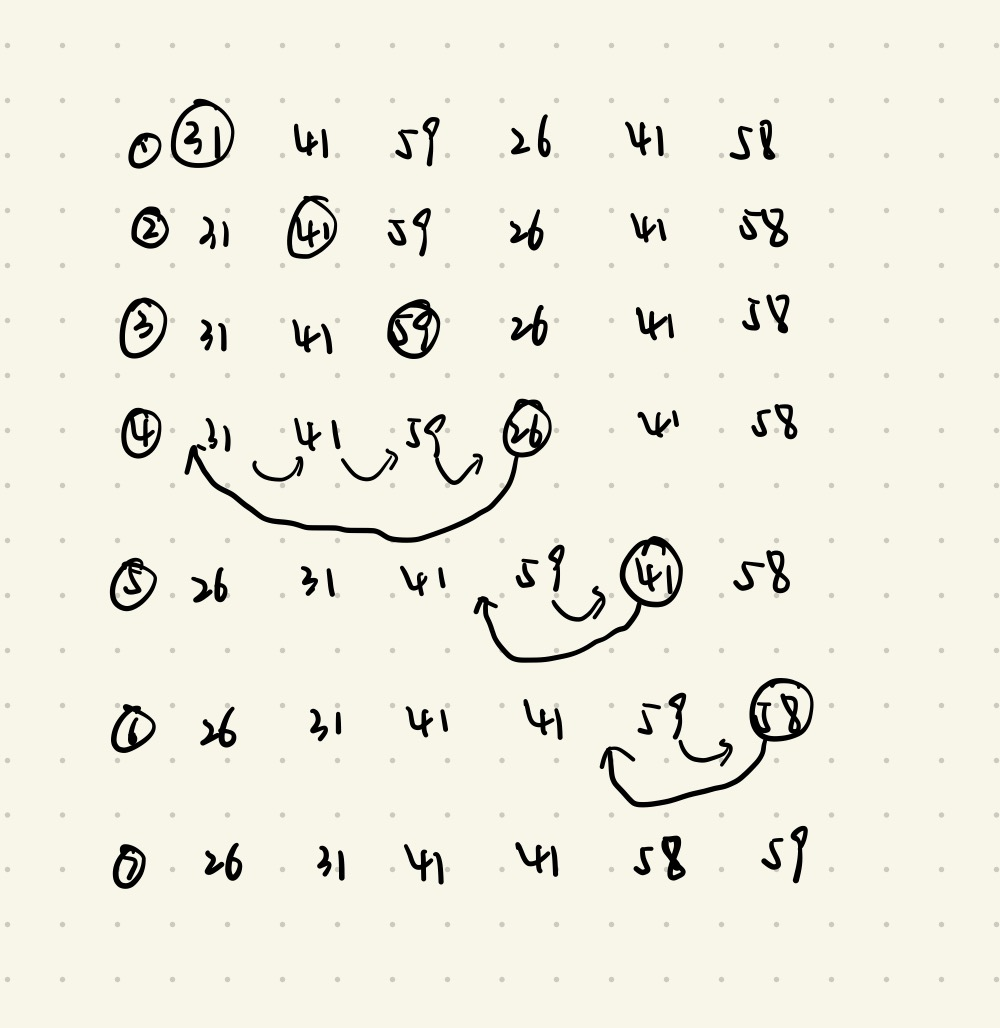
\includegraphics[scale=0.2]{sections/2/exercise2-1-1.jpeg}\\


\textbf{\textit{\Large{2.1-2}}}
\begin{lstlisting}[language=Python,numbers=left,numberstyle=\normalsize]
for j = 2 to A.length
    key = A[j]
    i = j -1 
    while i > 0 and A[i] < key
        A[i + 1] = A[i]
        i = i - 1
    A[i+1] = key
\end{lstlisting}


\textbf{\textit{\Large{2.1-3}}}
\begin{lstlisting}[language=Python,numbers=left,numberstyle=\normalsize]
#linear search
for i = 1 to A.length
    if v = A[i]:
        return i
return NIL
\end{lstlisting}


\textbf{\textit{\Large{2.1-4}}}\\
\\
\textbf{Input} : two integer arrays A and B such that $A.length=B.length=n$, and
$ \forall i \in \{0,2,\cdots,n-1\}, A[i],B[i] \in \{0,1\} $\\
\textbf{Output} : a integer array C such that $C.length=n+1$, and
$ \forall i \in \{0,\cdots,n\}, C[i]\in \{0,1\} $, and $c=a+b$, where a,b,c represents the decimal integers of A,B,C
\begin{lstlisting}[language=Python,numbers=left,numberstyle=\normalsize]
for i = n-1 to 0
    C[i] = (C[i+1] + A[i] + B[i]) / 2
    C[i+1] = (C[i+1] + A[i] + B[i]) % 2
return C
\end{lstlisting}
\subsection{Analyzing algorithms}
\subti{2.2-1}\\
$ \Theta(n^3) $\\


\subti{2.2-2}
\begin{lstlisting}[language=Python,numbers=left,numberstyle=\normalsize]
#selection sort
for i = 1 to A.length-1
    min = i
    for j = i+1 to A.length
        if A[j] < A[min]:
            min = j
    tmp=A[i]
    A[i]=A[min]
    A[min]=tmp
\end{lstlisting}
loop invatiant: the subarray $ A[1,\cdots,i-1] $ contains i-1 smallest elements and is sorted order\\
After selection sorting, $ A[n] $ is the largest element.\\
best-case: $ \Theta(n^2) $\\
worst-case: $ \Theta(n^2) $\\


\subti{2.2-3}\\
averange: $ (n+1) / 2 $ , running time: $ \Theta(n) $\\
worst case: $ n $ , running time: $ \Theta(n) $\\


\subti{2.2-4}\\
Set a standard input(denoted by A), check whether the input is the same as A, and output the standard output.

\subsection{Designing algorithms}
\subti{2.3-1}\\
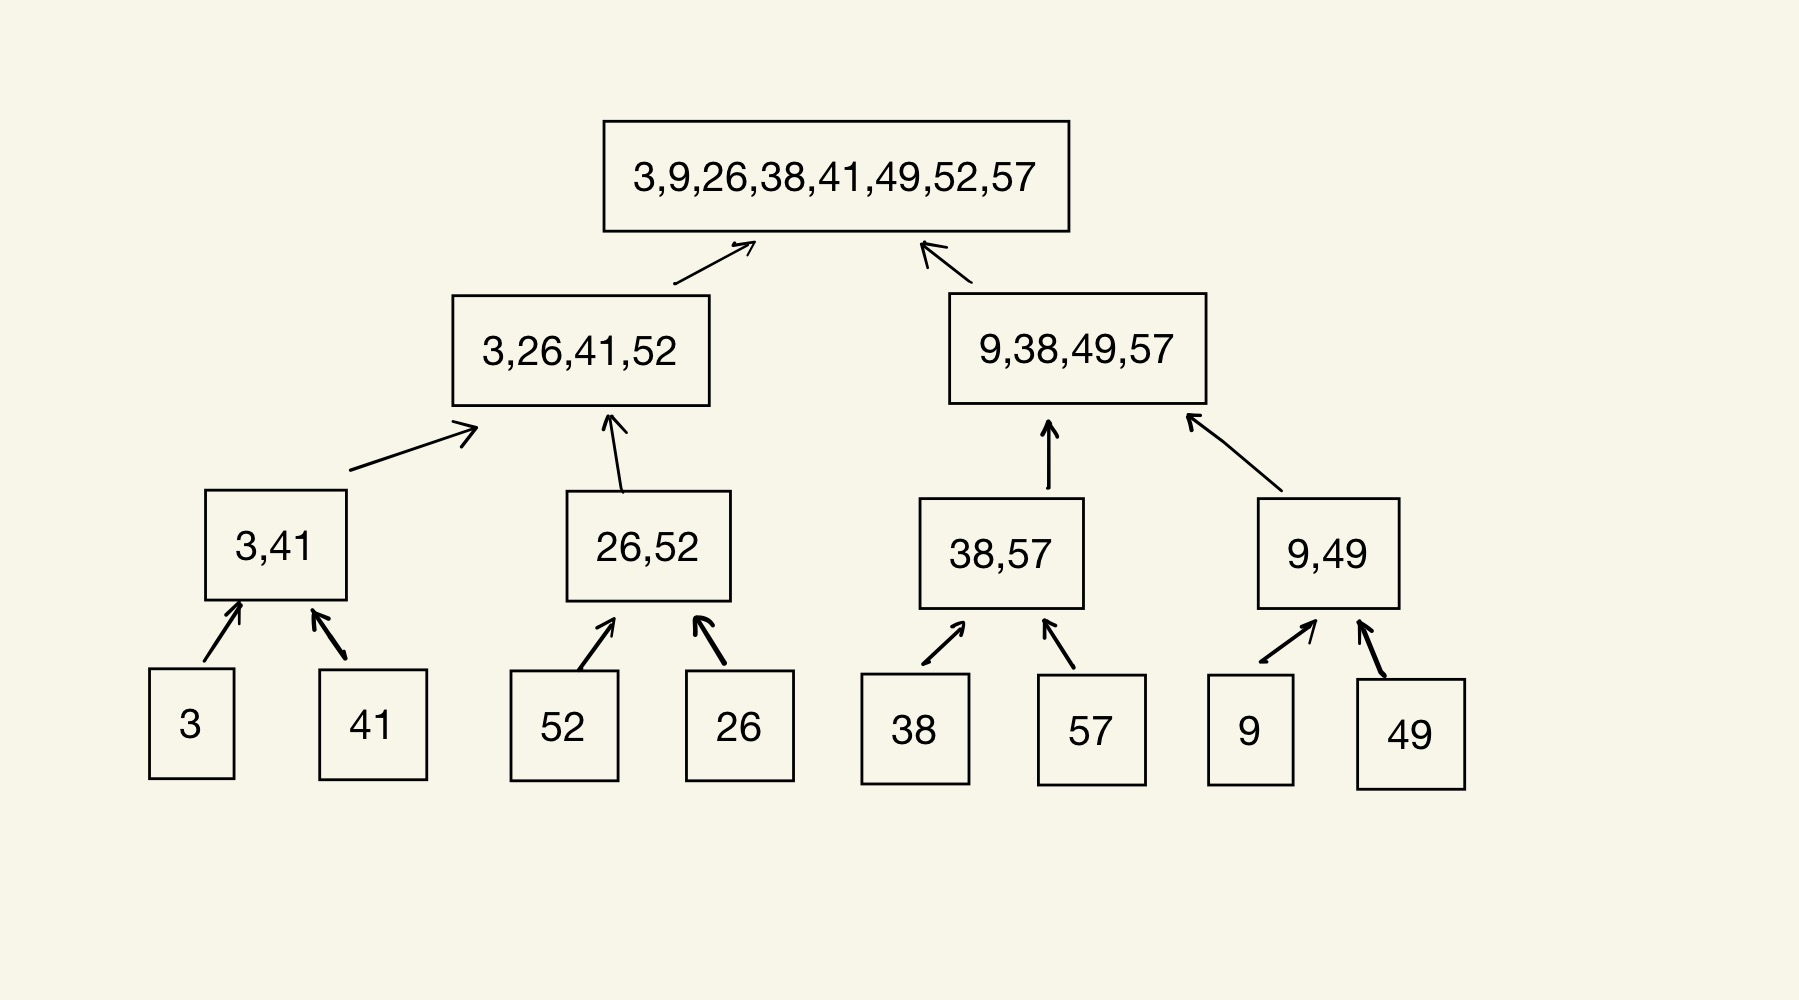
\includegraphics[scale=0.2]{sections/2/exercise2-3-1.jpeg}\\


\subti{2.3-2}
\begin{lstlisting}[language=Python,numbers=left,numberstyle=\normalsize]
MERGE(A,p,q,r):
    n1 = q - p + 1
    n2 = r - q
    let L[1 ... n1+1] and R[1 ... n2+1]
    for i = 1 to n1:
        L[i] = A[p + i - 1]
    for j = 1 to n2:
        R[j] = A[q + j]
    i = 1
    j = 1
    k = p
    while i < n1 and j < n2:
        if L[i] < R[j]:
            A[k] = L[i]
            i = i + 1
        else:
            A[k] = R[j]
            j = j + 1
        k = k + 1
    if i = n1:
        for t = j to n2:
            A[k] = R[j]
            j = j + 1
            k = k + 1
    else:
        for t = i to n1:
            A[k] = L[i]
            i = i + 1
            k = k + 1
MERGESORT(A,p,r):
    if p < r:
        q = [(p + r) / 2]
        MERGESORT(A,p,q)
        MERGESORT(A,q+1,r)
        MERGE(A,p,q,r)
\end{lstlisting}


\subti{2.3-3}\\
while $ n=2 $: $ T(2)=2=2\lg 2 $\\
while $ n=2^k , k>1 $:$ T(2^k)=2T(n/2)+n=(k-1)\cdot 2^k +2^k=k\cdot 2^k=n\lg n$\\
Q.E.D.\\


\subti{2.3-4}
\begin{align}
T(n)=\begin{dcases}
    1 & if n = 1\\
    T(n - 1) + n - 1 & if n > 1
\end{dcases}\notag
\end{align}


\subti{2.3-5}\\
binary search:
\begin{lstlisting}[language=Python,numbers=left,numberstyle=\normalsize]
binarysearch1(A,v):
    head = 1
    tail = A.length
    while head < tail :
        mid = (head + tail) / 2
        if v < A[mid]:
            tail = mid - 1
        else:
            head = mid
    return mid
\end{lstlisting}
Through binary searching, we guarantee that $ v $ occurs 
in an array that is half the length of the previous array.\\


\subti{2.3-6}\\
No. Even if we can use a binary search to simplify the searching part, 
the running time of moving $A[j]$ is still $\Theta(n^2)$


\subti{2.3-7}\\
First, we use merge-sort to sort S and we denote the ordered elements by $A[1\cdots,n]$.
The running time of merge-sort is $ \Theta(n \lg n) $.\\
Then, for $ i=1,2,\cdots,n-1 $, we use binary search to check whether there is
an element A[k] in $ A[i+1,\cdots,n] $ such that $ A[i]+A[k]=x $. Running time of this part is $ \Theta(n\lg n) $.\\
Thus, the running time of the algorithm is $\Theta(n\lg n)$


\subsection{Problems}


\end{document}